\chapter{Stand der Technik}
\label{chapter:Stand_der_Technik}
\myboxy{
	\begin{itemize}
		\item Bilder neu machen aus dem Schaltplan.
		\item Vector Controller, Funktionsweise nur kurz erklären und mehr auf die Anschlüsse eingehen.
		\item PIN-Mapping als Tabelle erstellen, für den Motor und den Vector Controller.
		\item QElectroTeck.
		\item PIN-Mapping als Tabelle erstellen, für den Motor und den Vector Controller.
		\item Auf die PDF verweisen.
	\end{itemize}
}{To-do}{\textwidth}



In dem folgenden Abschnitt werden die verwendeten Bauteile, welche in Kapitel \ref{chapter:Konzept} dargestellt worden sind, näher beschrieben.


\section{Antrieb – Golden Motor}
\label{section:Antrieb}

Golden Motor bietet eine Gesamtlösung bestehend aus einem BLDC-Motor und einem Vektor-Controller an. Der Motor wird dabei mit dem Controller verbunden, der eine Schnittstelle mit allen notwendigen Steuer- und Kontrollsignalen bereitstellt, um den Motor anzutreiben. Die Anschlüsse sowie die grundlegende Funktionsweise werden in den Abschnitten \ref{section:BLDC_Motor} und \ref{section:Vector_Controller} näher erläutert.



\subsection{BLDC Motor}
\label{section:BLDC_Motor}


Der in Abbildung \ref{BLDC_Motor:img:antrieb_motor} dargestellte BLDC-Motor verfügt über eine Leistung von 10 kW und kann optional durch eine Ölkühlung gekühlt werden, was jedoch für das Fahrzeug derzeit nicht relevant ist. Die Drehzahl ist variabel und kann zwischen 2.000 und 6.000 U/min eingestellt werden, mittls dem Vector Controller der in Abschnitt \ref{section:Vector_Controller} erklärt wird. Das Nenndrehmoment beträgt 26 Nm, während das maximale Drehmoment bei 85 Nm liegt. Der Wirkungsgrad des Motors beträgt 91 \% \cite{Golden_Motor:bldc_motor}.

\pagebreak[1]
\begin{figure}[!ht]
	\begin{center}
		\includegraphics[width=1\textwidth]{img/2_antrieb/motor_1.png}
		\caption{Golden Motor – 10 KW BLDC Motor Liquid Cooled}
		\label{BLDC_Motor:img:antrieb_motor}
	\end{center}
\end{figure}


Die Anschlüsse des Motors sind in Tabelle \ref{BLDC_Motor:tab:pinmapping} aufgelistet. Der Motor verfügt über zwei Hall-Sensor-Kabel, die jeweils drei Hall-Sensoren sowie einen Temperatursensor enthalten. Zusätzlich sind ein GND- und ein +5V-Versorgungsanschluss in den Hall-Sensor-Kabeln integriert. Die Spulen des Motors werden über sechs separate Kabel angeschlossen: U, V und W.
\pagebreak[1]
\begin{table}[!ht]
	\centering
	\caption{Pin Mapping – BLDC-Motor}
	\label{BLDC_Motor:tab:pinmapping}
	\begin{tabular}{lll}
		\hline
		\textbf{Anschluss}          & \textbf{Funktionalität} & \textbf{Farbe} \\ \hline
		\multicolumn{3}{c}{\textbf{Anschluss Adern Motor}}                     \\ \hline
		\multicolumn{1}{l|}{U1}     & Spule 1                 & Gelb           \\
		\multicolumn{1}{l|}{V1}     & Spule 2                 & Grün           \\
		\multicolumn{1}{l|}{W1}     & Spule 3                 & Blau           \\
		\multicolumn{1}{l|}{U2}     & Spule 1                 & Gelb           \\
		\multicolumn{1}{l|}{V2}     & Spule 2                 & Grün           \\
		\multicolumn{1}{l|}{W2}     & Spule 3                 & Blau           \\ \hline
		\multicolumn{3}{c}{\textbf{Motor Hall Kabel 1}}                        \\ \hline
		\multicolumn{1}{l|}{Hall A} & Hall Sensor             & Gelb           \\
		\multicolumn{1}{l|}{Hall B} & Hall Sensor             & Grün           \\
		\multicolumn{1}{l|}{Hall C} & Hall Sensor             & Blau           \\
		\multicolumn{1}{l|}{Temp}   & Temperatur Sensor       & Weiß           \\
		\multicolumn{1}{l|}{+5V}    & Spannungsversorgung     & Rot            \\
		\multicolumn{1}{l|}{GND}    & Masse                   & Schwarz        \\ \hline
		\multicolumn{3}{c}{\textbf{Motor Hall Kabel 2}}                        \\ \hline
		\multicolumn{1}{l|}{Hall A} & Hall Sensor             & Gelb           \\
		\multicolumn{1}{l|}{Hall B} & Hall Sensor             & Grün           \\
		\multicolumn{1}{l|}{Hall C} & Hall Sensor             & Blau           \\
		\multicolumn{1}{l|}{Temp}   & Temperatur Sensor       & Weiß           \\
		\multicolumn{1}{l|}{+5V}    & Spannungsversorgung     & Rot            \\
		\multicolumn{1}{l|}{GND}    & Masse                   & Schwarz        \\ \hline
	\end{tabular}
\end{table}
\pagebreak[4]



\subsubsection{Funktionsweise}
\label{BLDC_Motor:Funktionsweise}
Ein BLDC-Motor (Brushless DC Motor) unterscheidet sich grundlegend von einem herkömmlichen Gleichstrommotor. Während bei einem traditionellen DC-Motor die Polumschaltung (Kommutierung) mechanisch über Kohlebürsten erfolgt, übernimmt beim BLDC-Motor eine elektronische Steuerung diese Aufgabe. Dadurch entfällt die Notwendigkeit von Kohlebürsten, was den Motor effizienter und langlebiger macht\cite{mathworks:bldc_motor}.
\newpage



\subsection{Vector Controller}
\label{section:Vector_Controller}

Der Motor wird mithilfe eines Vektor-Controllers angesteuert, der in Abbildung \ref{Vector_Controller:img:Antrieb_Controller} dargestellt ist. Der Controller hat die Aufgabe, den Motor basierend auf den Eingangssignalen so zu steuern, dass beispielsweise eine gewünschte Drehzahl erreicht wird. Die genaue Funktionsweise des Vektor-Controllers wird kurz unter \ref{Vector_Controller:Funktionsweise} erläutert.

Das Pin-Mapping ist in Tabelle \ref{Vector_Controller:tab:pinmapping} aufgeführt. Bei den Steuersignalen muss auf den Spannungsbereich geachtet werden, da der Controller eine Störung meldet, wenn ein Signal außerhalb des zulässigen Bereichs liegt. Dies ist ein integriertes Sicherheitssystem des Controllers. Dies ist ein integriertes Sicherheitssystem des Controllers. So liegt beispielsweise bei der Bremse das digitale Signal bei 0, wenn die Spannung 1 V beträgt. Tritt ein Kabelbruch so wird die Spannung am Controller bei 0 V liegen und eine Warnung wird durch ein periodisches Piepen ausgegeben.


\begin{figure}[!ht]
	\begin{center}
		\includegraphics[width=1\textwidth]{img/2_antrieb/sine_1.png}
		\caption{Golden Motor – VECTOR 500 Motor Controller}
		\label{Vector_Controller:img:Antrieb_Controller}
	\end{center}
\end{figure}

\begin{table}[!ht]
	\centering
	\caption{Pin Mapping – Vector Controller}
	\label{Vector_Controller:tab:pinmapping}
	\begin{tabular}{lll|l}
		\hline
		\textbf{Anschluss}           & \textbf{Funktionalität}  & \textbf{Farbe}              & \textbf{U in V}             \\ \hline
		\multicolumn{4}{c}{\textbf{Batterie Eingang}}                                                                       \\ \hline
		\multicolumn{1}{l|}{B+}      & Versorgungsspannung      & RT                          & 48 V                        \\
		\multicolumn{1}{l|}{B-}      & Masse                    & SW                          & 0 V                         \\ \hline
		\multicolumn{4}{c}{\textbf{Motor Ausgnag}}                                                                          \\ \hline
		\multicolumn{1}{l|}{U}       & Spule 1                  & GE                          &                             \\
		\multicolumn{1}{l|}{V}       & Spule 2                  & GN                          &                             \\
		\multicolumn{1}{l|}{W}       & Spule 3                  & BL                          &                             \\ \hline
		\multicolumn{4}{c}{\textbf{Steuerungskabel}}                                                                        \\ \hline
		\multicolumn{1}{l|}{1}       & CANL - CAN-Bus           & \textcolor{red}{Vorhanden?} &                             \\
		\multicolumn{1}{l|}{2}       & CANH – CAN-Bus           & \textcolor{red}{Vorhanden?} &                             \\
		\multicolumn{1}{l|}{3}       & Motor Temperatur         & BL                          &                             \\
		\multicolumn{1}{l|}{4, 5, 6} & Masse                    & SW                          & 0 V                         \\
		\multicolumn{1}{l|}{7}       & Tempomat                 & Gr                          & 0 V - 5 V                   \\
		\multicolumn{1}{l|}{10}      & Elektronisches Schloss   & OR                          & 0 V - 5 V                   \\
		\multicolumn{1}{l|}{11}      & Hall C – Sensor          & BL                          &                             \\
		\multicolumn{1}{l|}{12}      & Hall B – Sensor          & GN                          &                             \\
		\multicolumn{1}{l|}{13}      & Hall A – Sensor          & GE                          &                             \\
		\multicolumn{1}{l|}{14}      & +5 V                     & RT                          & 5 V                         \\
		\multicolumn{1}{l|}{15}      & +12V Bremse              & GN\&WS                      & \textcolor{red}{Vorhanden?} \\
		\multicolumn{1}{l|}{16}      & Bremse                   & BL\&WS                      & 1 V - 5 V                   \\
		\multicolumn{1}{l|}{20}      & Hohe Geschwindigkeit     & BL                          & \textcolor{red}{Vorhanden?} \\
		\multicolumn{1}{l|}{21}      & Masse                    & SW                          & 0 V                         \\
		\multicolumn{1}{l|}{24}      & Niedrige Geschwindigkeit & BL                          & \textcolor{red}{Vorhanden?} \\
		\multicolumn{1}{l|}{25}      & Masse                    & SW\&WS                      & 0 V                         \\
		\multicolumn{1}{l|}{26}      & Gaspedal                 & GN\&WS                      & 1 V - 5 V                   \\
		\multicolumn{1}{l|}{27}      & Masse                    & SW                          & 0 V                         \\ \hline
	\end{tabular}
\end{table}
\pagebreak[4]

\subsubsection{Funktionsweise}
\label{Vector_Controller:Funktionsweise}
Der Vektor-Controller verwendet die Motorsteuerungstechnologie der feldorientierten Regelung (Field-Oriented Control, FOC). Dabei wird die Position des Rotors im Motor mithilfe von Hall-Sensoren ermittelt. Mit der FOC-Technik ist es möglich, das Verhältnis von Drehmoment pro Ampere zu maximieren. Dafür muss der Rotorflussvektor im rechten Winkel (90 Grad) zum Statorflussvektor ausgerichtet sein \cite{Golden_Motor:Vector_Controller}.


\newpage


\section{Echtzeitfähige Steuerung – Speedgoat}
\label{section:speedgoat}
\myboxy{
	\begin{itemize}
		\item I/O Module 691 zuende Erklären.
	\end{itemize}
}{To-do}{\textwidth}

Der Baseline Real-Time Target Machine, wie in Abbildung \ref{speedgoat:img:steuerung_goat} dargestellt, ist ein echtzeitfähiges System. Es wird hauptsächlich in der Entwicklung und beim Testen von komplexen Steuerungs- und Regelungssystemen eingesetzt, bei denen die Echtzeitfähigkeit eine zentrale Rolle spielt.\\
Echtzeitfähigkeit bezieht sich auf die Fähigkeit eines Systems, innerhalb einer festgelegten Frist auf externe Ereignisse oder Eingaben zu reagieren. In der Informatik und Technik spricht man von einem Echtzeitsystem, wenn es

rechtzeitig arbeiten muss. Die Reaktionszeit auf Ereignisse ist hierbei entscheidend, da Verzögerungen zu Fehlern oder unvorhersehbaren Zuständen führen könnten \cite{DIN_44300}.

\pagebreak[1]
\begin{figure}[!ht]
	\begin{center}
		\includegraphics[width=1\textwidth]{img/2_steuerung/goat_1.png}
		\caption{Speedgoat – Baseline Real-Time Target Machine}
		\label{speedgoat:img:steuerung_goat}
	\end{center}
\end{figure}
\pagebreak[1]

Speedgoat-Systeme integrieren sich nahtlos mit Simulink, einer Software von MathWorks, die häufig zur Modellierung und Simulation dynamischer Systeme verwendet wird. Dank einer breiten Palette an I/O-Modulen lassen sich verschiedene Sensoren und Aktuatoren problemlos an die Systeme anschließen.
Echtzeitsysteme von Speedgoat sind Computer, die in der Lage sind, Aufgaben innerhalb festgelegter Zeitintervalle auszuführen. Diese Systeme sind entscheidend für Anwendungen, bei denen die zeitliche Genauigkeit eine große Bedeutung ist, wie beispielsweise bei der Steuerung von Motoren, der Regelung von Prozessen oder der Simulation von physikalischen Systemen.


\pagebreak[1]
\begin{figure}[!ht]
	\begin{center}
		\includegraphics[width=1\textwidth]{img/2_steuerung/goat_2.png}
		\caption{Speedgoat – Ansicht der Modulanschlüsse}
		\label{speedgoat:img:Modulanschlüsse}
	\end{center}
\end{figure}
\pagebreak[1]
In Abbildung \ref{speedgoat:img:Modulanschlüsse} sind die Anschlüsse der I/O-Module des Speedgoat-Systems dargestellt. Die Zuordnung der Module zu den entsprechenden Anschlüssen ist in Tabelle \ref{speedgoat:tab:Module} ersichtlich.

Das Modul IO397-50k-50k kann über ein Sensor-Aktor-Kabel von Phoenix Contact extern angeschlossen werden, wie in Abbildung \ref{IO397_50k:img:Module} dargestellt.
Zusätzlich wird das Modul IO691 mittels eines 9-Pin D-Sub-Steckers angeschlossen.
\pagebreak[1]
\begin{table}[!ht]
	\centering
	\caption{Speedgoat – Anschlüsse der Module}
	\label{speedgoat:tab:Module}
	\begin{tabular}{clll}
		\hline
		\multicolumn{2}{c}{\textbf{I/O Module}} & \multicolumn{1}{c}{\textbf{Name}} & \textbf{Funktion}               \\ \hline
		\multirow{2}{*}{1}                      & \multicolumn{1}{l|}{A}            & IO397-50k         & analog I/O  \\
		                                        & \multicolumn{1}{l|}{B}            & IO397-50k         & digital I/O \\ \hline
		\multirow{2}{*}{2}                      & \multicolumn{1}{l|}{A}            & IO691             & CAN         \\
		                                        & \multicolumn{1}{l|}{B}            & IO691             & CAN         \\ \hline
		\multirow{2}{*}{3}                      & \multicolumn{1}{l|}{A}            & IO397-50k         & analog I/O  \\
		                                        & \multicolumn{1}{l|}{B}            & IO397-50k         & digital I/O \\ \hline
		\multirow{2}{*}{4}                      & \multicolumn{1}{l|}{A}            & Frei              &             \\
		                                        & \multicolumn{1}{l|}{B}            & Frei              &             \\ \hline
	\end{tabular}
\end{table}
\pagebreak[4]




\subsection{I/O-Modul – IO397-50k}
\label{section:IO397_50k}

Das in Abbildung \ref{IO397_50k:img:Module} gezeigte IO397-50k I/O-Modul bietet eine Vielzahl von analogen und digitalen Ein- und Ausgängen. Die Anschlüsse werden auf Modul A, das die analogen Schnittstellen bereitstellt, und Modul B, welches die digitalen Schnittstellen umfasst, verteilt. Die Anschlussbelegung werden in den Tabellen \ref{IO397_50k:tab:Board_A} und \ref{IO397_50k:tab:Board_B} dargestellt. Die Spannungen der Ein- und Ausgänge können softwaregesteuert angepasst werden \cite{speedgoat:IO397_50k}.

\pagebreak[1]
\begin{figure}[!ht]
	\begin{center}
		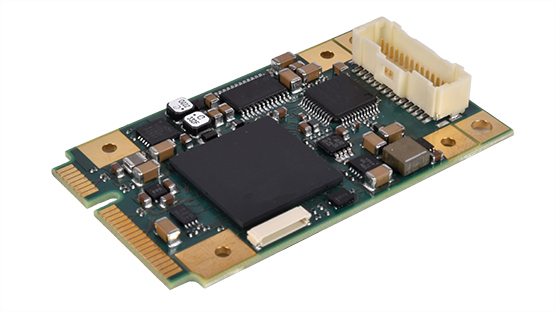
\includegraphics[width=0.7\textwidth]{img/2_steuerung/goat_io397.png}
		\caption{Speedgoat – I/O Module 397 \cite{speedgoat:IO397_50k}}
		\label{IO397_50k:img:Module}
	\end{center}
\end{figure}
\pagebreak[1]

\subsubsection{Pin Mapping – IO397-50k}


Das Terminal Board A ist für die Verarbeitung analoger Signale konzipiert, sowohl für Eingänge als auch für Ausgänge. Die Tabelle \ref{IO397_50k:tab:Board_A} zeigt das Pin-Mapping von Terminal Board A. Dieses Board verfügt über Anschlüsse für insgesamt vier analoge Eingänge (Pins A1 bis A8) und vier analoge Ausgänge (Pins A9 bis A12). Die Ausgänge sind an einen Digital-zu-Analog-Wandler (DAC) angeschlossen, während die Eingänge mit einem Analog-zu-Digital-Wandler (ADC) verbunden sind.

\pagebreak[1]
\begin{table}[!ht]
	\centering
	\caption{IO397-50k Pin Mapping – Terminal Board A: analog I/O \cite{speedgoat:IO397_50k}}
	\label{IO397_50k:tab:Board_A}
	\begin{tabular}{lll}
		\hline
		\textbf{Pin}             & \textbf{Funktionalität} & \textbf{Type} \\ \hline
		\multicolumn{1}{l|}{A1}  & Analog input 1 +        & ADC           \\
		\multicolumn{1}{l|}{A2}  & Analog input 1 -        & ADC           \\
		\multicolumn{1}{l|}{A3}  & Analog input 2 +        & ADC           \\
		\multicolumn{1}{l|}{A4}  & Analog input 2 -        & ADC           \\
		\multicolumn{1}{l|}{A5}  & Analog input 3 +        & ADC           \\
		\multicolumn{1}{l|}{A6}  & Analog input 3 -        & ADC           \\
		\multicolumn{1}{l|}{A7}  & Analog input 4 +        & ADC           \\
		\multicolumn{1}{l|}{A8}  & Analog input 4 -        & ADC           \\ \hline
		\multicolumn{1}{l|}{A9}  & Analog output 1         & DAC           \\
		\multicolumn{1}{l|}{A10} & Analog output 2         & DAC           \\
		\multicolumn{1}{l|}{A11} & Analog output 3         & DAC           \\
		\multicolumn{1}{l|}{A12} & Analog output 4         & DAC           \\ \hline
		\multicolumn{1}{l|}{A13} & GND                     & GND           \\
		\multicolumn{1}{l|}{A14} & GND                     & GND           \\
		\multicolumn{1}{l|}{A15} & 0 V                     & 0 V           \\
		\multicolumn{1}{l|}{A16} & 5 V DC                  & 5 V DC        \\
		\multicolumn{1}{l|}{A17} & GND                     & GND           \\
		\multicolumn{1}{l|}{SH}  & SH                      & Shielding     \\ \hline
	\end{tabular}
\end{table}
\pagebreak[1]


Terminal Board B hingegen bietet eine flexible Konfiguration für digitale Ein- und Ausgänge. Die Tabelle \ref{IO397_50k:tab:Board_B} zeigt das Pin Mapping von Terminal Board B. Die Pins B3 bis B16 sind für konfigurierbare I/O-Funktionalitäten ausgelegt und nutzen TTL-Signale (Transistor-Transistor-Logik), was sie besonders für schnelle digitale Schaltvorgänge geeignet macht. Dieses Board ermöglicht es, die Anschlüsse flexibel zu nutzen, je nach den Anforderungen der Applikation. Auch hier gibt es mehrere Spannungs- und Ground-Anschlüsse, sowie eine Abschirmung (Shielding) für das M12-Kabel, um elektromagnetische Störungen zu minimieren.


\pagebreak[1]
\begin{table}[!ht]
	\centering
	\caption{IO397-50k Pin Mapping – Terminal Board B: analog I/O \cite{speedgoat:IO397_50k}}
	\label{IO397_50k:tab:Board_B}
	\begin{tabular}{lll}
		\hline
		\textbf{Pin}             & \textbf{Funktionalität} & \textbf{Type} \\ \hline
		\multicolumn{1}{l|}{B1}  & 0 V                     & 0 V           \\
		\multicolumn{1}{l|}{B2}  & 5 V DC                  & 5 V DC        \\ \hline
		\multicolumn{1}{l|}{B3}  & I/O 0                   & IN/OUT        \\
		\multicolumn{1}{l|}{B4}  & I/O 1                   & IN/OUT        \\
		\multicolumn{1}{l|}{B5}  & I/O 2                   & IN/OUT        \\
		\multicolumn{1}{l|}{B6}  & I/O 3                   & IN/OUT        \\
		\multicolumn{1}{l|}{B7}  & I/O 4                   & IN/OUT        \\
		\multicolumn{1}{l|}{B8}  & I/O 5                   & IN/OUT        \\
		\multicolumn{1}{l|}{B9}  & I/O 6                   & IN/OUT        \\
		\multicolumn{1}{l|}{B10} & I/O 7                   & IN/OUT        \\
		\multicolumn{1}{l|}{B11} & I/O 8                   & IN/OUT        \\
		\multicolumn{1}{l|}{B12} & I/O 9                   & IN/OUT        \\
		\multicolumn{1}{l|}{B13} & I/O 10                  & IN/OUT        \\
		\multicolumn{1}{l|}{B14} & I/O 11                  & IN/OUT        \\
		\multicolumn{1}{l|}{B15} & I/O 12                  & IN/OUT        \\
		\multicolumn{1}{l|}{B16} & I/O 13                  & IN/OUT        \\\hline
		\multicolumn{1}{l|}{B17} & GND                     & GND           \\
		\multicolumn{1}{l|}{B18} & SH                      & Shielding     \\ \hline
	\end{tabular}
\end{table}
\pagebreak[4]

\newpage
\subsection{I/O-Modul – IO691}
\label{section:IO691}

Das IO691 I/O-Modul bietet eine intelligente CAN-Schnittstelle mit zwei Kanälen, die sowohl flexible Datenrate CAN (CAN FD) als auch High-Speed CAN (CAN HS) unterstützen. Es ist kompatibel mit CAN 2.0A/B-Netzwerken und unterstützt SAE J1939 sowie ASAM XCP für Bypassing. Alle Signale sind über 9-polige D-Sub-Front-CAN-Anschlüsse zugänglich \cite{speedgoat:IO691}.

\pagebreak[1]
\begin{figure}[!ht]
	\begin{center}
		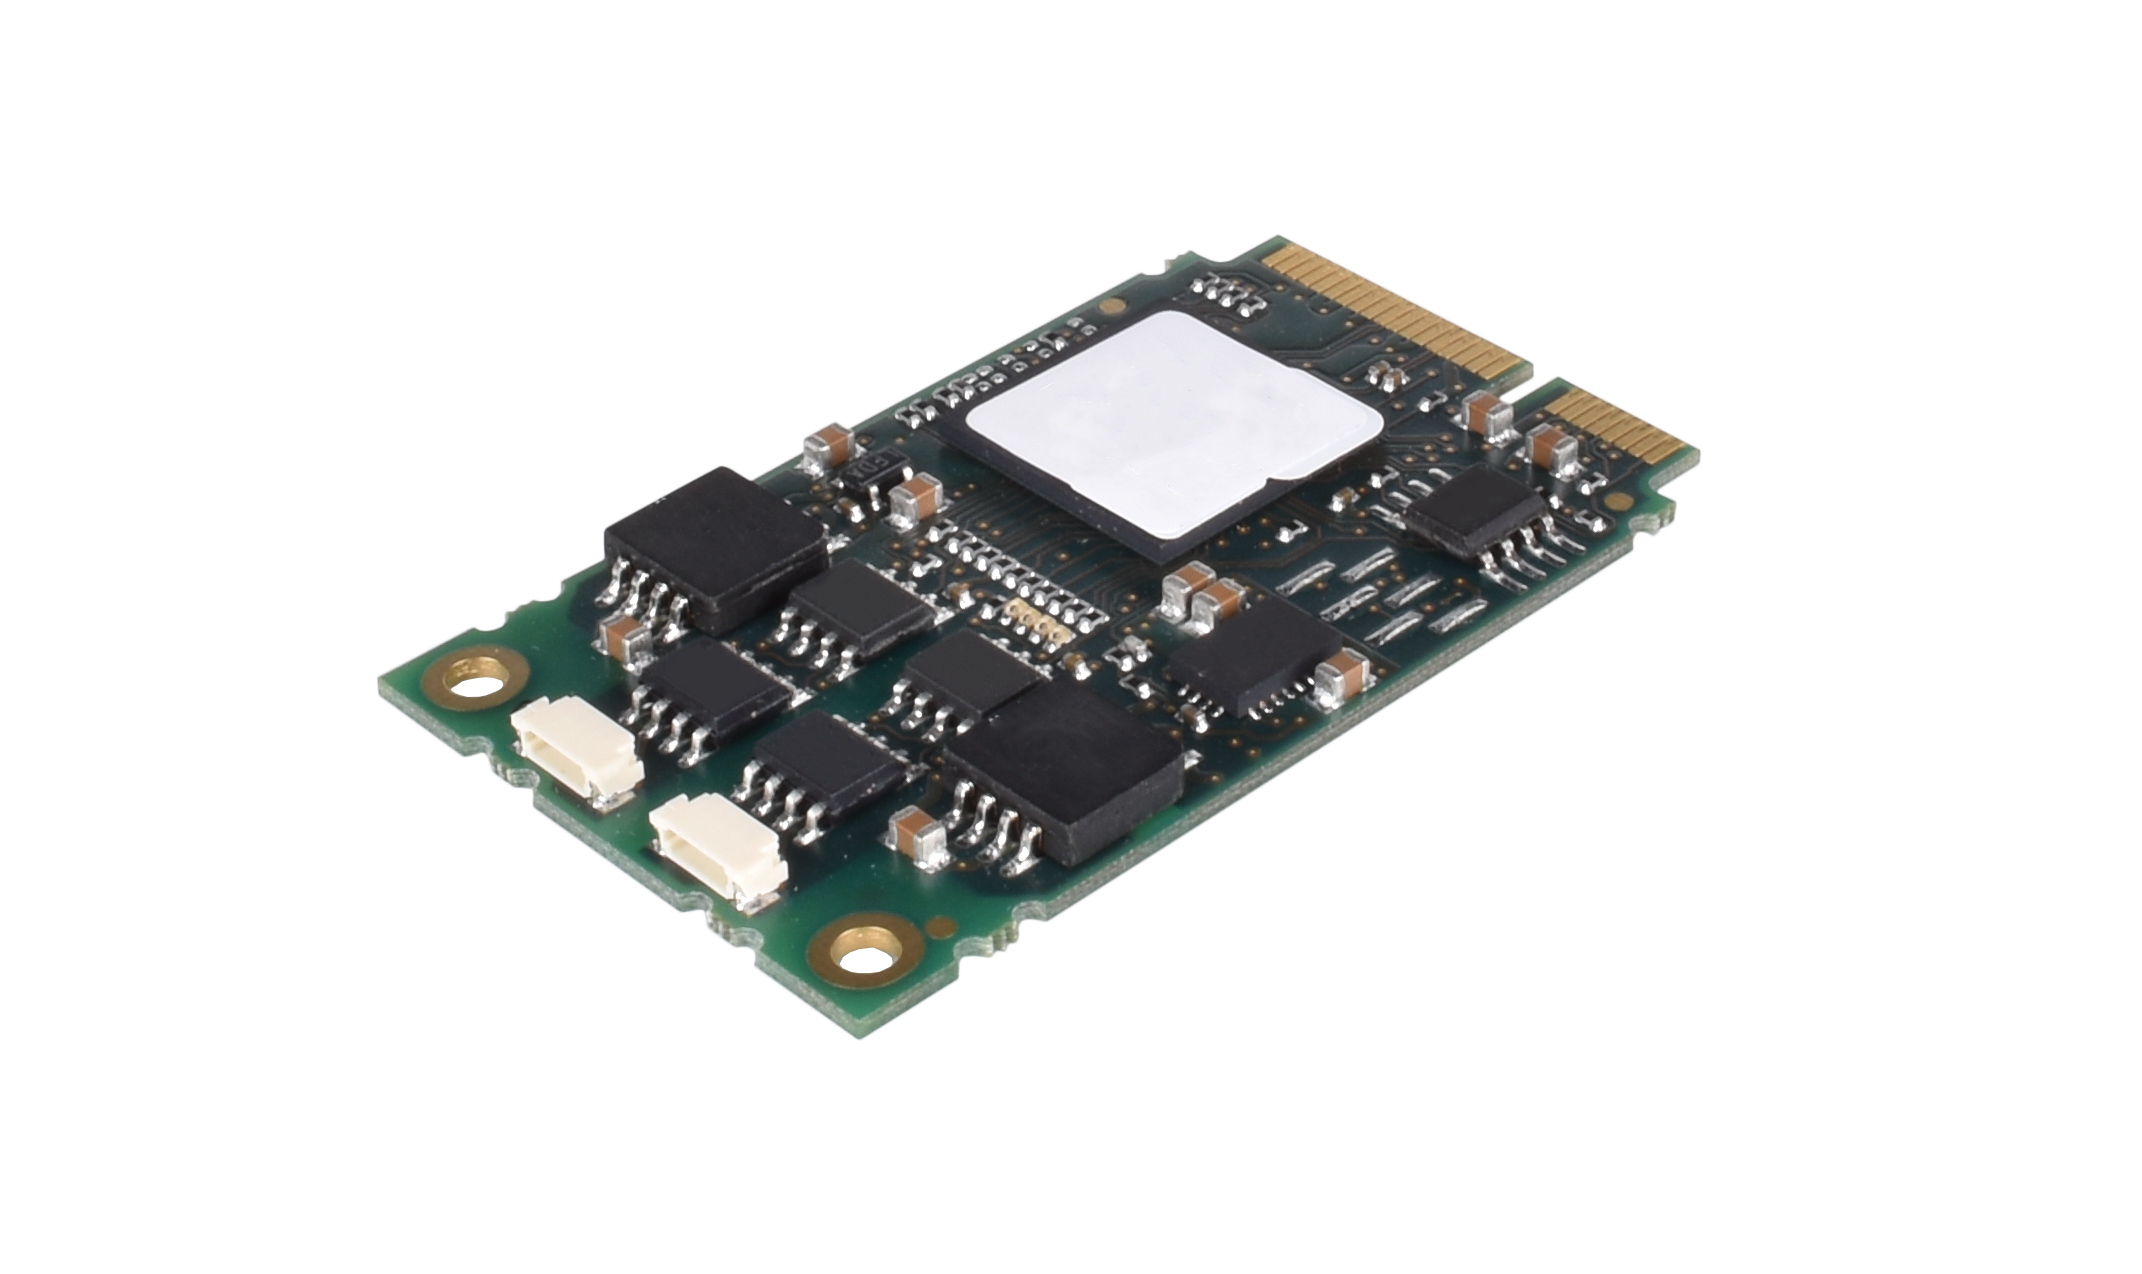
\includegraphics[width=0.7\textwidth]{img/2_steuerung/goat_io691.png}
		\caption{Speedgoat – I/O Module 691 \cite{speedgoat:IO691}}
		\label{img_2_2:goat:IO691}
	\end{center}
\end{figure}
\pagebreak[4]




\subsubsection{Pin Mapping –  IO691}

\pagebreak[1]
\begin{table}[!ht]
	\centering
	\caption{IO691 Pin Mapping}
	\label{speedgoat:IO691}
	\begin{tabular}{ll}
		\hline
		\textbf{Pin}           & \textbf{DB9 Connector A/B, Signal} \\ \hline
		\multicolumn{1}{l|}{1} & -                                  \\
		\multicolumn{1}{l|}{2} & CAN-low                            \\
		\multicolumn{1}{l|}{3} & GND                                \\
		\multicolumn{1}{l|}{4} & -                                  \\
		\multicolumn{1}{l|}{5} & -                                  \\
		\multicolumn{1}{l|}{6} & GND                                \\
		\multicolumn{1}{l|}{7} & CAN-high                           \\
		\multicolumn{1}{l|}{8} & -                                  \\
		\multicolumn{1}{l|}{9} & -                                  \\ \hline
	\end{tabular}
\end{table}
\pagebreak[4]


\newpage
\section{Simulink}
\label{section:Simulink}

\myboxy{
	\begin{itemize}
		\item
	\end{itemize}
}{To-do}{\textwidth}


\subsection{IO397-50k Module Konfigurieren}
\label{Simulink:IO397_50k_Konfigurieren}
In dem Driver Block, wie in Abbildung \ref{IO397_50k_Konfigurieren:img:Driver_Block} können die Pull-Resitors des Modules eingestellt werden, die in der Tabelle \ref{IO397_50k_Konfigurieren:tab:Pull_Resistors} aufgelistet sind.

\pagebreak[1]
\begin{figure}[!ht]
	\begin{center}
		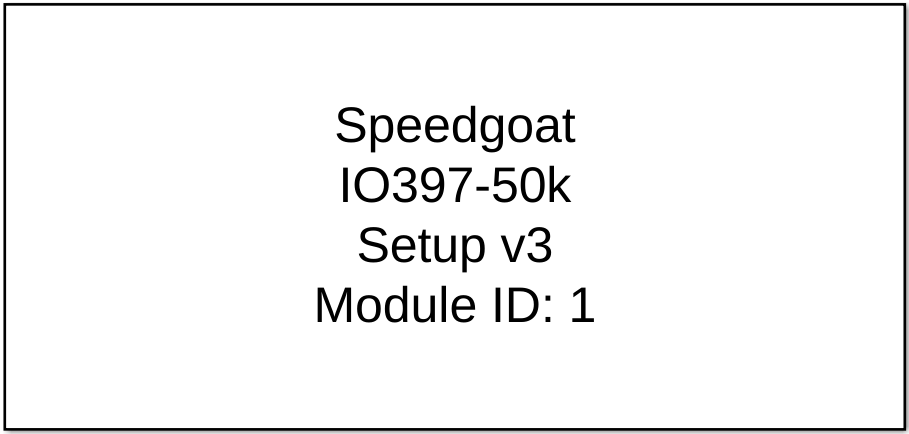
\includegraphics[width=0.7\textwidth]{img/4_simulink/IO397_50k.png}
		\caption{Simulink – Driver Block – IO397-50k}
		\label{IO397_50k_Konfigurieren:img:Driver_Block}
	\end{center}
\end{figure}
\pagebreak[1]

Pull-Resistors werden verwendet um saubere Digitale schaltzustände zu erhalten, es gibt drei unterschiedliche Zustände, hight, low und floating die unterschieden werden.

\pagebreak[1]
\begin{table}[!ht]
	\centering
	\caption{Simulink – Pull Resistors}
	\label{IO397_50k_Konfigurieren:tab:Pull_Resistors}
	\begin{tabular}{ll}
		\hline
		\textbf{Modus}                         & \textbf{Funktion} \\ \hline
		\multicolumn{1}{l|}{pull-up 3,3V}      &                   \\
		\multicolumn{1}{l|}{weak pull-up 5,0V} &                   \\
		\multicolumn{1}{l|}{pull-down}         &                   \\
		\multicolumn{1}{l|}{floating}          &                   \\ \hline
	\end{tabular}
\end{table}
\pagebreak[1]

\pagebreak[1]
\begin{figure}[ht!]
	\centering
	\begin{circuitikz}
		\ctikzset{resistor = european}
		\draw[R={Pullup-Resistor}](9.0,-5.5)to(9.0,-3.5);
		\draw[short={}](11.5,-5.5)to(11.5,-5.5);
		\draw[nos={S1}](9.0,-8.0)to(9.0,-6.5);
		\draw[short={}](9.0,-6.5)to(9.0,-5.5);
		\draw[short={}](9.0,-6.0)to(11.5,-6.0);
		\draw[short={}](9.0,-8.0)to(9.0,-8.5);
		\draw[short={}](8.5,-8.5)to(9.5,-8.5);
		\draw(9.0,-3.5)to(9.0,-3.0) node[diamondpole]{};
		\draw(9.0,-3.0)to(9.0,-3.0) node[diamondpole]{.          U+};
		\draw[short={ UND}](11.5,-5.5)to(11.5,-7.5);
		\draw[short={}](11.5,-7.0)to(11.0,-7.0);
		\draw[short={}](11.5,-5.5)to(13.0,-5.5);
		\draw[short={}](13.0,-5.5)to(13.0,-7.5);
		\draw[short={}](13.0,-7.5)to(11.5,-7.5);
		\draw[short={Q}](13.0,-6.5)to(14.0,-6.5);
	\end{circuitikz}
	\caption{Schaltung – Pullup Resistors}
	\label{IO397_50k_Konfigurieren:img:Pullup Resistors}
\end{figure}
\pagebreak[4]

\pagebreak[1]
\begin{figure}[ht!]
	\centering
	\begin{circuitikz}
		\ctikzset{resistor = european}
		\draw[R={Pulldown-Resistor}](9.0,-8.0)to(9.0,-6.5);
		\draw[short={}](11.5,-5.5)to(11.5,-5.5);
		\draw[nos={S1}](9.0,-5.5)to(9.0,-3.5);
		\draw[short={}](9.0,-6.5)to(9.0,-5.5);
		\draw[short={}](9.0,-6.0)to(11.5,-6.0);
		\draw[short={}](9.0,-8.0)to(9.0,-8.5);
		\draw[short={}](8.5,-8.5)to(9.5,-8.5);
		\draw(9.0,-3.5)to(9.0,-3.0) node[diamondpole]{};
		\draw(9.0,-3.0)to(9.0,-3.0) node[diamondpole]{.          U+};
		\draw[short={ UND}](11.5,-5.5)to(11.5,-7.5);
		\draw[short={}](11.5,-7.0)to(11.0,-7.0);
		\draw[short={}](11.5,-5.5)to(13.0,-5.5);
		\draw[short={}](13.0,-5.5)to(13.0,-7.5);
		\draw[short={}](13.0,-7.5)to(11.5,-7.5);
		\draw[short={Q}](13.0,-6.5)to(14.0,-6.5);
	\end{circuitikz}
	\caption{Schaltung – Pullup Resistors}
	\label{IO397_50k_Konfigurieren:img:Pulldown Resistors}
\end{figure}
\pagebreak[4]




\subsection{IO691 Module Konfigurieren}
\label{Simulink:IO691_Konfigurieren}




\newpage
\section{QElectroTech}
\label{section:QElectroTech}

\myboxy{
	\begin{itemize}
		\item
	\end{itemize}
}{To-do}{\textwidth}



